\section{Restructuring of the Conceptual Schema} 

\subsection{Redundancy Analysis}

No redundancies were found in the original schema of figure \ref{img:diagram}.

\subsection{Restructured ER Schema}

See Figure \ref{img:diagram_rest} on next page.

\subsection{Data Dictionary}

\subsubsection{New entities and relationships}
\label{sec:dictionary-rest}

 One new entity and two new relationships are added to the original \hyperref[sec:dictionary]{data dictionary}. They originate from the multivalued and composite attribute \texttt{Stop[name]} and from the elimination of ISA between \texttt{Stop} and \texttt{Platform}.
 
 For the stop name, a modular approach was followed. In particular, the fact that the number of translations is not fixed, but can change over time was considered. This has lead to the following table, where each translation is associated with the corresponding language.

\begin{table}[htp]
	\centering
	\begin{tabularx}{\columnwidth}{|c|C|c|c|}
		\hline
		\textbf{Entity} & \textbf{Description} & \textbf{Attributes} & \textbf{Identifiers} \\
		\hline
		\textbf{StopName} & Translation of a stop name & language, value & \{language, value\} \\
		\hline
	\end{tabularx}
	\caption{Newly-added entities}\label{tbl:entites-rest}
\end{table} 

\begin{table}[htp]
	\centering
	\begin{tabularx}{\columnwidth}{|C|C|C|c|C|}
		\hline
		\textbf{Relationship} & \textbf{Description} & \textbf{Components} & \textbf{{\footnotesize Attributes}} & \textbf{Identifiers} \\
		\hline
		\textbf{stopHasName} & Connects the translations of the stop name of a line to the stop itself & Stop, StopName & - & \{latitude, longitude, language, value\} \\ \hline
		\textbf{ISA-S-P} & Relationship connecting a platform to the corresponding stop tuple & Stop, Platform & - & \{latitude, longitude\} \\ 
		\hline
	\end{tabularx}
	\caption{Newly-added relationships}\label{tbl:relationships-rest}
\end{table}

\subsubsection{New External Constraints}

No new external constraints were added.

\begin{landscape}
	\begin{figure}[htb]
		\thispagestyle{plain}
		\centering
		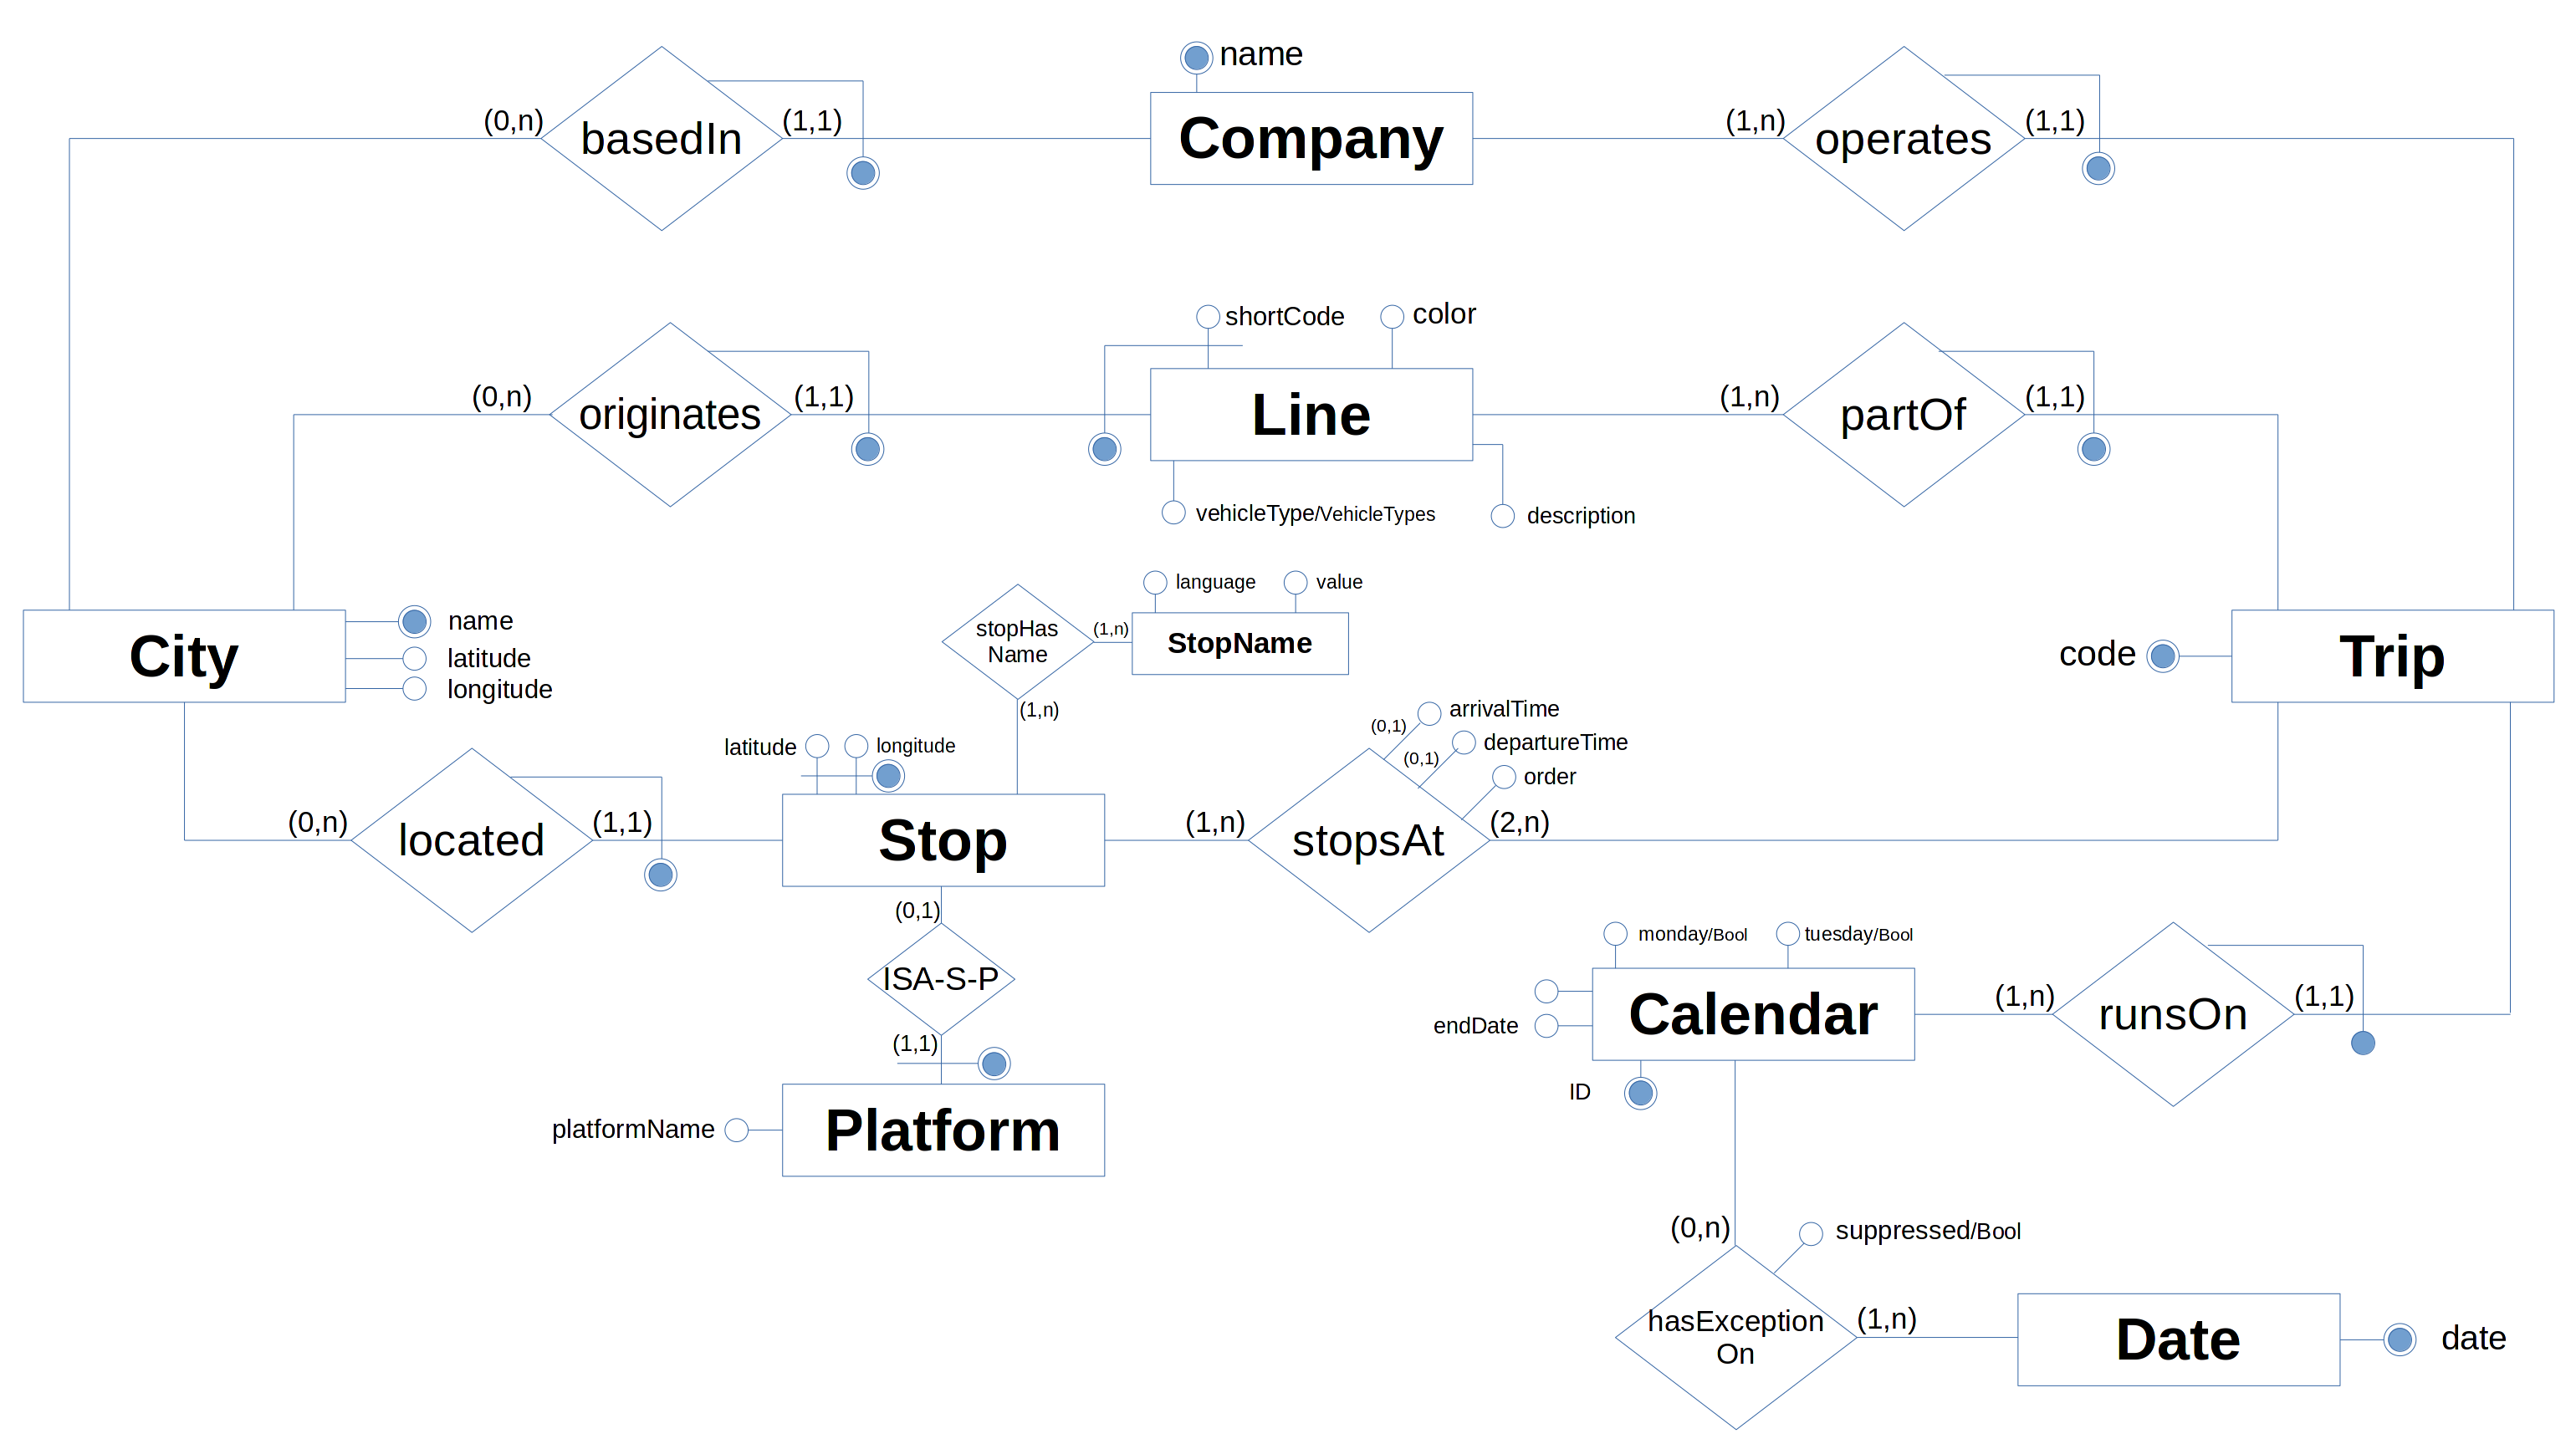
\includegraphics[height=\textheight]{diagram_rest}
		\caption{Restructured ER Schema \\ {\footnotesize \textit{Note: not all attributes have been indicated in the schema. Please check the \hyperref[sec:dictionary-rest]{data dictionary} for a complete overview}}}\label{img:diagram_rest}
	\end{figure}
\end{landscape}

\subsection{Reformulated Application Load}

	The following data is based on the original \hyperref[tbl:volumes]{table of volumes} and on the \hyperref[sec:assumptions]{assumptions}, particularly on point 4 about the translations. Regarding access tables, costs were written by considering the worst possible scenario (i.e. the one with maximal computational expense).

	\subsubsection{Table of Volumes}
	
	\begin{table}[h]
		\centering
		\begin{tabular}{|c|c|c|}
			\hline
			\textbf{Concept} & \textbf{Construct} & \textbf{Volume} \\
			\hline
			City & Entity & 30 \\ \hline
			Stop & Entity & 75 \\ \hline
			StopName & Entity & 150 \\ \hline
			Platform & Entity & 20 \\ \hline
			Trip & Entity & 500 \\ \hline
			Company & Entity & 5 \\ \hline
			Line & Entity & 25 \\ \hline
			Calendar & Entity & 10 \\ \hline
			Date & Entity & 200 \\ \hline
			basedIn & Relationship & 5 \\ \hline
			operates & Relationship & 500 \\ \hline
			originates & Relationship & 25 \\ \hline
			partOf & Relationship & 500 \\ \hline
			located & Relationship & 100 \\ \hline
			stopsAt & Relationship & 4500 \\ \hline
			runsOn & Relationship & 500 \\ \hline
			hasExceptionOn & Relationship & 150 \\ \hline
			stopHasName & Relationship & 150 \\ \hline
			ISA-S-P & Relationship & 30 \\ \hline
		\end{tabular}
		\caption{Restructured Table of Volumes}\label{tbl:volumes-rest}
	\end{table}

	\newpage
	\subsubsection{Access Tables}
	
	\paragraph{(1)} Get a list of \textit{(maximum)} ten stops with name in a specific language matching the user-given string
	
	\begin{table}[h!]
		\centering
		\begin{tabular}{|c|c|c|c|}
			\hline
			\textbf{Concept} & \textbf{Construct} & \textbf{Accesses} & \textbf{Type} \\
			\hline
			StopName & Entity & 75 & Read \\ \hline
			stopHasName & Relationship & 10 & Read \\ \hline
			Stop & Entity & 10 & Read \\ \hline 
			ISA-S-P & Relationship & 10 & Read \\ \hline
			Platform & Entity & 10 & Read \\ \hline
			located & Relationship & 10 & Read \\ \hline
			City & Entity & 10 & Read \\ \hline
		\end{tabular}
		\caption{Access table for operation 1}\label{tbl:access-1}
	\end{table}

	\paragraph{(2)} Get a list of \textit{(maximum)} ten stops with name in a specific language that are contained in a set of coordinates
	
	\begin{table}[h!]
		\centering
		\begin{tabular}{|c|c|c|c|}
			\hline
			\textbf{Concept} & \textbf{Construct} & \textbf{Accesses} & \textbf{Type} \\
			\hline
			Stop & Entity & 75 & Read \\ \hline 
			stopHasName & Relationship & 10 & Read \\ \hline
			StopName & Entity & 10 & Read \\ \hline
			located & Relationship & 10 & Read \\ \hline
			City & Entity & 10 & Read \\ \hline
			ISA-S-P & Relationship & 10 & Read \\ \hline
			Platform & Entity & 10 & Read \\ \hline
		\end{tabular}
		\caption{Access table for operation 2}\label{tbl:access-2}
	\end{table}

	\newpage
	\paragraph{(3)} Find the next ten trips, with line and company information, that depart from a specific stop at a given date and time \textit{(assuming that the stop coordinates are known)}

	\begin{table}[h!]
		\centering
		\begin{tabular}{|c|c|c|c|}
			\hline
			\textbf{Concept} & \textbf{Construct} & \textbf{Accesses} & \textbf{Type} \\
			\hline
			stopsAt & Relationship & 15 & Read \\ \hline
			Trip & Entity & 15 & Read \\ \hline
			runsOn & Relationship & 15 & Read \\ \hline
			Calendar & Entity & 15 & Read \\ \hline
			hasExceptionOn & Relationship & 225 & Read \\ \hline
			Date & Relationship & 225 & Read \\ \hline
			partOf & Relationship & 10 & Read \\ \hline
			Line & Entity & 10 & Read \\ \hline
			operates & Relationship & 10 & Read \\ \hline
			Company & Entity & 10 & Read \\ \hline
		\end{tabular}
		\caption{Access table for operation 3}\label{tbl:access-3}
	\end{table}

	\paragraph{(4)} Find the next ten trips departing from one stop and arriving at another one, at a given date and time \textit{(assuming that the stop coordinates are known)}
 
	\begin{table}[h!]
		\centering
		\begin{tabular}{|c|c|c|c|}
			\hline
			\textbf{Concept} & \textbf{Construct} & \textbf{Accesses} & \textbf{Type} \\
			\hline
			stopsAt & Relationship & 30 & Read \\ \hline
			Trip & Entity & 30 & Read \\ \hline
			runsOn & Relationship & 30 & Read \\ \hline
			Calendar & Entity & 30 & Read \\ \hline
			hasExceptionOn & Relationship & 225 & Read \\ \hline
			Date & Relationship & 225 & Read \\ \hline
			partOf & Relationship & 10 & Read \\ \hline
			Line & Entity & 10 & Read \\ \hline
			operates & Relationship & 10 & Read \\ \hline
			Company & Entity & 10 & Read \\ \hline
		\end{tabular}
		\caption{Access table for operation 4}\label{tbl:access-4}
	\end{table}

	\newpage
	\paragraph{(5)} Add a new company given the name and the headquarter city, \textit{and considering that all possible cities are already loaded into the database}
	
	\begin{table}[h!]
		\centering
		\begin{tabular}{|c|c|c|c|}
			\hline
			\textbf{Concept} & \textbf{Construct} & \textbf{Accesses} & \textbf{Type} \\
			\hline
			City & Entity & 1 & Read \\ \hline
			Company & Entity & 1 & Write \\ \hline 
			basedIn & Relationship & 1 & Write \\ \hline
		\end{tabular}
		\caption{Access table for operation 5}\label{tbl:access-5}
	\end{table}

	\paragraph{(6)} Add a new line given short code, color, type of vehicle and city, \textit{and considering that all possible cities are already loaded into the database}
	\begin{table}[h]
		\centering
		\begin{tabular}{|c|c|c|c|}
			\hline
			\textbf{Concept} & \textbf{Construct} & \textbf{Accesses} & \textbf{Type} \\
			\hline
			City & Entity & 1 & Read \\ \hline
			Line & Entity & 1 & Write \\ \hline
			originates & Relationship & 1 & Write \\ \hline
		\end{tabular}
		\caption{Access table for operation 6}\label{tbl:access-6}
	\end{table}

	\paragraph{(7)} Add a new trip given the code, the timetable, the operating company and the calendar
	\begin{table}[h]
		\centering
		\begin{tabular}{|c|c|c|c|}
			\hline
			\textbf{Concept} & \textbf{Construct} & \textbf{Accesses} & \textbf{Type} \\
			\hline
			Trip & Entity & 1 & Write \\ \hline
			stopsAt & Relationship & 9 & Write \\ \hline
			partOf & Relationship & 1 & Write \\ \hline
			operates & Relationship & 1 & Write \\ \hline
			runsOn & Relationship & 1 & Read \\ \hline
		\end{tabular}
		\caption{Access table for operation 7}\label{tbl:access-7}
	\end{table}

	\paragraph{(8)} Modify the schedule for a calendar knowing its code (add one exceptional date)
	\begin{table}[h!]
		\centering
		\begin{tabular}{|c|c|c|c|}
			\hline
			\textbf{Concept} & \textbf{Construct} & \textbf{Accesses} & \textbf{Type} \\
			\hline
			hasException & Relationship & 1 & Write \\ \hline
			Date & Entity & 1 & Write \\ \hline
		\end{tabular}
		\caption{Access table for operation 8}\label{tbl:access-8}
	\end{table}